\documentclass[a4paper]{article}
\usepackage[T1]{fontenc}
\usepackage{listings}
\usepackage{adjustbox}
\usepackage[english]{babel}
\usepackage[utf8]{inputenc}
\usepackage{lmodern}
\usepackage{subfig}
\usepackage{xcolor}
\usepackage{graphicx}
\usepackage{amsmath}
\usepackage{amssymb}
\usepackage{float}
\usepackage{mathtools}
\usepackage{algorithm2e}
\usepackage{hyperref}
\usepackage{tikz}
\usetikzlibrary{arrows}
\lstset{
  belowcaptionskip=1\baselineskip,
  breaklines=true,
  frame=L,
  xleftmargin=\parindent,
  language=Matlab,
  showstringspaces=false,
  basicstyle=\footnotesize\ttfamily,
  keywordstyle=\bfseries\color{green!40!black},
  commentstyle=\itshape\color{purple!40!black},
  identifierstyle=\color{blue},
  stringstyle=\color{orange},
  columns=flexible,
}

\begin{document}
\title{\vspace{-4cm}Blockchain summer school - Maersk study case}
\author{Marius-Florin Cristian (wdx186)}
\maketitle

\newcommand{\E}[1]{\mathbb{E}\left\{#1\right\}}
\newcommand{\heads}{\textsc{heads}}
\newcommand{\tails}{\textsc{tails}}
\newcommand{\ld}{\log_2}
\newcommand{\ceil}[1]{\left\lceil#1\right\rceil}

\newcommand{\code}[1]{\texttt{#1}}
\renewcommand{\Pr}[1]{\mathbb{P}\left\{#1\right\}}
\newcommand{\sumin}{\sum_{i=1}^n}
\newcommand{\sumi}[1]{\sum_{i=1}^{#1}}
\newcommand{\N}{\mathcal{N}}
\newcommand{\Rn}{\mathbb{R}^n}
\newcommand{\Rnn}{\mathbb{R}^{n \times n}}
\newcommand{\Rmn}{\mathbb{R}^{m \times n}}
\newcommand{\Rmm}{\mathbb{R}^{m \times m}}
\renewcommand{\min}[1]{\underset{#1}{\text{min}}}
\renewcommand{\max}[1]{\underset{#1}{\text{max}}}
\newcommand{\B}{\mathbf{B}}
\newcommand{\Binv}{\mathbf{B}^{-1}}
\newcommand{\x}{\mathbf{x}}
\newcommand{\gfx}{\nabla f(x)}
\newcommand{\gfk}{\nabla f_k}
\newcommand{\gfkT}{\nabla f_k^T}
\newcommand{\parans}[1]{\left(#1\right)}
\newcommand{\lambdamin}[1]{\lambda_\text{min}\left(#1\right)}
\newcommand{\gbg}{g_k^T B_k g_k}
\newcommand{\pc}{p_k^C}
\newcommand{\alphac}{\alpha^C}
\newcommand{\normg}{\lVert g_k \rVert}
\newcommand{\norm}[1]{\lVert #1 \rVert}
\newcommand{\rank}[1]{\text{rank}\left\{#1\right\}}
\newcommand{\st}{\text{ s.t. }}

\section{Abstract}
This paper will explore three solutions for the problem of storing and keeping financial data synchronised across the subsidiaries of a large company, with the possibility of granting an outside entity limited access to it such that the validity of the data can be agreed on.\\
The next chapters present an instance of the problem, a solution from a centralised perspective, a distributed ledger perspective, and a blockchain perspective, with regard to the advantages and disatvantages of each particular case.

\section{The problem}
\href{http://www.maersk.com}{A.P. Moller - Maersk} and it's subsidiaries deal with a large amount of transactions across multiple countries each days. Governments usually have different tax policies and sanctions towards (unintentional) tax fraud (such as omitted data or human error).\\
Currently the accounting is split amongst subsidiaries, and even if subsidiary $S_1$ initiaties a transaction, subsidiary $S_2$ can add extra acounting information that might be needed or not when submitting a tax report in country $C_1$.\\
\\
At the current state the handling of data is done manually in Excell for each subsidiary, and uses an Enterprise Resource Planning (ERP) system to keep track of everything. This process takes time, and for example in Spain the time interval for submitting the monthly tax report is four days, in Romania, they need to check the validity of the reports submitted by tracking the history of how the data was modified over time (wich is not possible in the current system and thus sanctions are applied). Even more at any point in time, any governamental entity can perform a check of all the reports submitted in an interval up to five or ten years and needs to track how they were modified. Another obstacle is that, this data should not be visible to everybody, such that two subsidiaries should not be able to access or modify all of the data, just the one that is intended to.\\
\\
\subsection{The flow}
Let $t$ denote one transaction and it's data (such as sender, value, receiver, sender\_country, receiver\_country, currency...)\\ 
Let $S=\{S_0,S_1,...\}$ the set of subsidiaries (we can treat them as different databases), where $S_i$ contains either all of a transactions data, or partial data.\\
Let $T_i=\{(t_i,S_{j},S_{j+1},S_{j+2},...)\}$ be the mapping of a transaction $t_i$ over the subsidiaries that contains data related to it.\\ 
Let $C=\{C_0,C_1,C_2...\}$ be the set of countries in which tax report must be filled in.\\
Let $T_{C_i}=\{T_0, T_1,...\}$ be the set of transactions that need to be submited for a ceratain country $C_i$ in order to pay tax.\\
\\
The flow of a transaction record in the current system:\\
First a transaction $t_0$ is registered by subsidiary $S_0$, $T_0=\{(t_0,S_0)\}$ will be present in the ERP. This initial state should be always immutable. $S_1$ adds extra data fields to $t_0$, for example $extra\_charges,\ country$ that concatenates extra expenses. The ERP will now contain $T_0=\{(t_0,S_0,S_1)\}$. Let's assume that $S_2$ needs to pay the tax for the current cumulative value of $t_0$, therefore it will make a request to ERP, and ERP will provide the transaction data from $S_0$ and from $S_1$ and submit it to the country $C_1's$ tax authority. ERP will mark $t_0$ as paid. If $S_4$ wants to add extra charges, or a bank fee, or alter the data for overpaying it, this will be added in the ERP after the moment of transaction such that $T_0=\{(t_0,S_0,S_1,S_4)\}$. But the tax is already marked as paid, and the extra modification might be considered tax evasion.\\
Because the data is not immutable, mistakes are sometimes made, and data might disappear; let's take the case of accidental deletion of $t_0$ in $S_0$ (an employee of subsidiary 0 deletes the Excel row containing the transaction), now when the tax authority does the validation, the missing data can be considered as tax evasion.\\
\\
The flow is exemplified in the following graph
\begin{center}
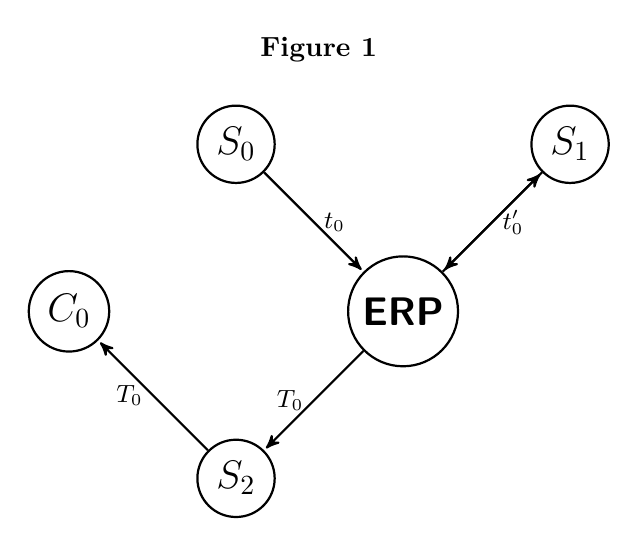
\begin{tikzpicture}[->,>=stealth',shorten >=1pt,auto,node distance=3cm,
                    thick,main node/.style={circle,draw,font=\sffamily\Large\bfseries}]

  \node[main node] (1) {ERP};
  \node[main node] (2) [above left of=1] {$S_0$};
  \node[main node] (3) [below left of=1] {$S_2$};
  \node[main node] (4) [above right of=1] {$S_1$};
  \node[main node] (5) [above left of=3] {$C_0$};

  \path[every node/.style={font=\sffamily\small}]
    (1) edge node [left] {$T_0$} (3)
    	edge node [left] {} (4)
    (2) edge node [right] {$t_0$} (1)
    (3) edge node [left] {$T_0$} (5)
    (4) edge node [right] {$t_0'$} (1);
    
\node[align=center,font=\bfseries, yshift=2em] (title) 
    at (current bounding box.north)
    {Figure 1};

\end{tikzpicture}

\end{center}

\section{A centralised point of view}
In the current scheme, the ERP system is the central authority, that deals with the manangement of data from subsidiaries (we can treat it as a special join table from a relational database that also contains the privilege level of its subsidiaries). The main concerns are: the data is not immutable on each of the subsidiaries and the subsidiaries might be out of sync. Thus a request can return either "not found", invalid data or valid data. Making the transactions immutable solves the "not found" branch, but there is no feasible way to distinguish between invalid and valid data.\\

\subsection{Immutable data}
The first step is to ensure that data cannot dissapear. Implementing a database (with timestamped operations) at node (subsidiary) level, that can only Read, Create and Update guarantees that the data will not be accidentally deleted. The timestamp ensures that the transactions can be traced back in time, and that there can be set a priority protocol, such that the modifications must be in chronological order. What if there are two ongoing modifications (each on different subsidiaries) that are interdependent, how would this affect the validity of the data?
\subsection{Keeping data in sync}
Besides the timestamp, the second step is to introduce a locking mechanism, to ensure the validity of the interdependent data. This would be done at ERP level as follows:\\
Every operation at node level is forced to report back to the ERP the type of operation and the timestamp and in the case of a requested Update operation, it must wait for all of the other Update operations to finish. This will create a bottleneck, as not all of the data is interdependant. A better approach would be to implement a locking protocol on attribute (collumn in the database) level, but this would be very hard to keep track of, especially that the data is not handled at transaction level, but bundles of transactions.\\
Besides the initial permission protocol, now there is a locking protocol at ERP level as well.\\
\subsection{Bundles of transactions}
At individual transaction level:\\
The CREATE operation, just instantiates a new transaction, therefore it is considered safe (the worst case is when dealing with offline transactions, that need to be added manually by a human, as they might misstype it). The READ operation is also considered safe, as it does not modify the state. If a transactions data is under modification in the locking table, it can also be marked with a read-warning flag. Our main concern is the UPDATE operation. The modifications are done asynchronously, thus when commiting them there might be a conflict (another entity commited a new version before the current one was submitted), thus it should not be accepted, because it's validity is questionable.\\
\\
When dealing with bundles of transactions there should be a merge protocol defined at the ERP level, such that it will only commit and update the timestamps of the transactions that are valid for sure, and return back to the node the ones that failed. The node then has to READ the data again, and apply the modifications again to the transactions that had discrepancies between the two reads. Hopefully this will not be a frustrating process for the person who edits the data, as it can be tuned at interface level, and the volume might not be that big. This paper cannot make further analysis on the topic as some facts are not known.\\
\subsection{Conclusion}
This might provide a good starting point as there are no major security flaws on the system level, it assumes a certain level of automatization (transactions are stored automatically when a payement is done through the system), everything is closed, only humans can decide what to do with the data (leak it or not). It is possible to trace back a transaction back in time, and provide a full report on how it was modified, but there are still some questions:\\
What if a subsidiary dissapears, or because of natural reasons, it loses it's data storage? Should there be a replication mechanism?\\
A tax authority might not trust this hermetic system.\\
The timestamps can be forged.\\
The volume of transactions might be too big and it might take too much time to keep track of the modification; there is a big bottleneck at ERP level, with each node (subsidiary) that wants to modify the same data.\\
\section{Distributed Ledger solution}
In this chapter we will explore a distributed ledger technology (DLT) approach, that tries to enchance the centralised solution, and solve some of its weaknesses but maintain the strenghts.\\
\begin{center}
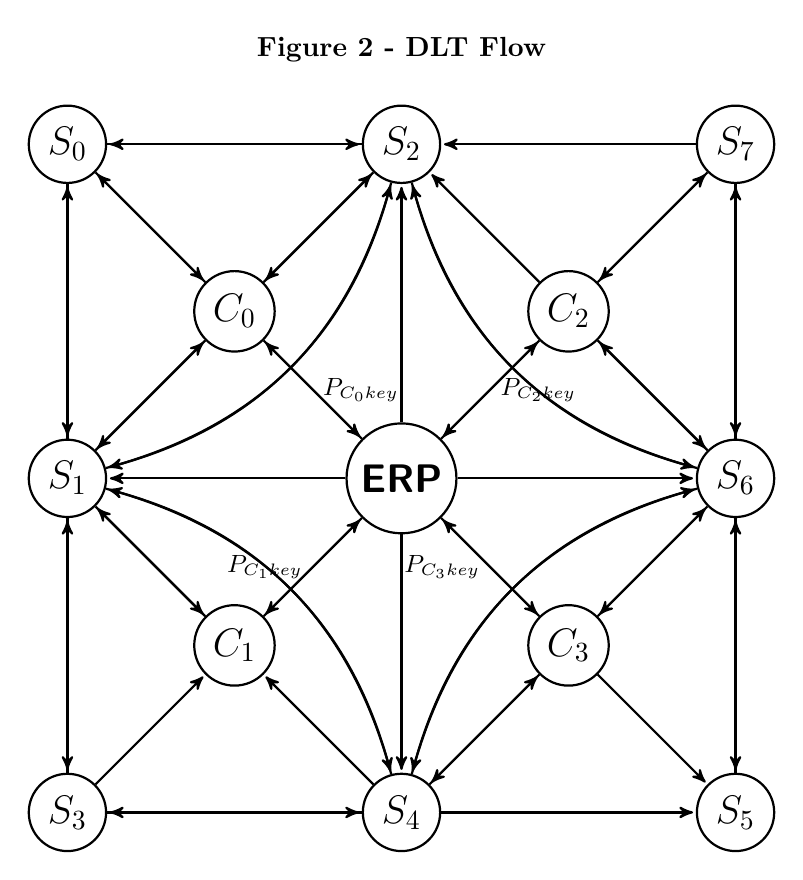
\begin{tikzpicture}[->,>=stealth',shorten >=1pt,auto,node distance=3cm,
                    thick,main node/.style={circle,draw,font=\sffamily\Large\bfseries}]

  \node[main node] (1) {ERP};
  \node[main node] (2) [above left of=1] {$C_0$};
  \node[main node] (3) [below left of=1] {$C_1$};
  \node[main node] (4) [above right of=1] {$C_2$};
  \node[main node] (5) [below right of=1] {$C_3$};
  \node[main node] (6) [above left of=2] {$S_0$};
  \node[main node] (7) [below left of=2] {$S_1$};
  \node[main node] (8) [above right of=2] {$S_2$};
  \node[main node] (9) [below left of=3] {$S_3$};
  \node[main node] (10) [below right of=3] {$S_4$};
  \node[main node] (11) [below right of=5] {$S_5$};
  \node[main node] (12) [above right of=5] {$S_6$};
  \node[main node] (13) [above right of=4] {$S_7$};

  \path[every node/.style={font=\sffamily\small}]
    (1) edge node {} (2)
    	edge node {} (3)
    	edge node {} (4)
    	edge node {} (5)
    	edge node {} (7)
    	edge node {} (8)
    	edge node {} (10)
    	edge node {} (12)
    (6) edge node {} (2)
    	edge node {} (7)
    	edge node {} (8)
    (7) edge node {} (6)
    	edge node {} (2)
    	edge node {} (3)
    	edge node {} (9)
    	edge [bend right] node {} (8)
    	edge [bend left] node {} (10)
    (3) edge node {} (7)
    (8) edge node {} (6)
    	edge node {} (2)
    	edge [bend left] node {} (7)
    	edge [bend right] node {} (12)
    (9) edge node {} (10)
    	edge node {} (7)
    	edge node {} (3)
    (10)edge node {} (3)
    	edge node {} (9)
    	edge node {} (11)
    	edge [bend right] node {} (7)
    	edge [bend left] node {} (12)
    	edge node {} (5)
    (5) edge node {} (11)
    	edge node {} (10)
    	edge node {} (12)
    (12)edge node {} (5)
    	edge [bend left] node {} (8)
    	edge [bend right] node {} (10)
    	edge node {} (4)
    	edge node {} (13)
    	edge node {} (11)
    (11)edge node {} (12)	
    (4) edge node {} (12)
    	edge node {} (13)
    	edge node {} (8)
    (13)edge node {} (4)
    	edge node {} (8)
    	edge node {} (12)		
    (2) edge node [right] {$P_{C_0 key}$} (1)
    	edge node {} (6)
    	edge node {} (7)
    	edge node {} (8)
    (3) edge node [left] {$P_{C_1 key}$} (1)
    (4) edge node [right] {$P_{C_2 key}$} (1)
    (5) edge node [left] {$P_{C_3 key}$} (1);
    
\node[align=center,font=\bfseries, yshift=2em] (title) 
    at (current bounding box.north)
    {Figure 2 - DLT Flow};

\end{tikzpicture}

\end{center}
\subsection{The Flow}
The problem is modeled as a graph of fully connected subgraphs. There are 4 types of nodes: a Permission node, Regulator nodes, Super nodes and Normal nodes. Each subraph uses a distributed ledger for storing data, and the graph to emit events in the form of hashes of the data.\\
\\
The Permission node: Represents the permission authority, that indicates what data is restricted to other nodes. The permission node is connected to all of the Regulator nodes and Super nodes, such that it can broadcast policy updates into the network. To ensure that the Regulator nodes are trusted, verified, and do not try to access data that is prohibited to them, the Permission node certifies them with a cryptographic key that is used to gain read access just to the data that is strictly under their authority. In Figure 2, the permission node is markes as "ERP"\\
\\
Regulator nodes: Represented by the tax autorithy in each country. In the network they are the center of each cluster of fully connected graphs, and are connected to every type of node (except Regulator nodes, as the current design does not explore sharing data between governments, it would be a nice future study case). Their role is to check and agree on the validity of the data, thus they represent an important part in the consensus mechanism, and are considered as trusted supervisors. If they get corrupt, data leakages are at risk. Because the corporate entity does not trust the Regulator nodes, it is up to the Super nodes to supervise them, provide fault detection (to some extent) against such entities and expose them. The Regulator and the Super nodes represent the core of this design flow. In Figure 2, the Regulator nodes are: $\{C_0,C_1,C_2,C_3\}$.\\
\\
Super nodes: Represented by the subsidiaries that have to report to more than one tax authority (we can think of them as "Border Subsidiaries" that deal with transactions across multiple countries). They represent the bridges between fully connected graphs, and they are connected to the Permission node, any number of Regulator nodes, and \textbf{all} of the nodes (normal or super) in each fully connected graph. For example if a super node $S$ is part of $C_0$ and $C_1$'s graph, them being fully connected graphs, then by definition $S$ is connected to every node in those graphs. In Figure 2, the Super nodes are: $\{S_1, S_2, S_6, S_4\}$ A super node has 3 propreties:\\
1) A super node broadcasts the policy updates and permissions of the ERP to the other nodes (such that each normal node "hears" the policy that takes effect over it);\\
2) Any 2 super nodes that share a common tax authority can contest any sanctions (with proof) on the tax authorities side.\\
3) A super node may become a normal node and vice versa.\\
\\
Normal nodes: Represented by the subsidiaries that only deal with transactions in a single country. Thus only report to a single authority. They keep a distributed ledger with permissions (replicated database), whos state is shared in a peer-to-peer network only between the nodes that are part of it's current fully connected graph. In Figure 2 the normal nodes are $\{S_0,S_3,S_7,S_5\}$.\\
\subsection{The consensus}
A detailed technical solution of the consensus is presented in Leemon Bairds paper\cite{hashgraph}.\\
\\
Let $G$ be the network graph, and $G_{C_i}$ a fully connected subgraph of G, that revolves arround Regulator node $C_i$. There is a distributed ledger for each subgraph $G_{C_i}$ in the graph, and the role of the subgraph is to ensure that every member knows every event.\\
The first type of consensus is the one that validates each transaction and modification of it. The regulator keeps an updated copy of the networks "ledger" (in this case not reffering to the database, but the signatures history), and is also part in the \textbf{virtual voting} (as presented in "The Swirlds Hashgraph Consensus Algorithm" - Chapter 4\cite{hashgraph}) process of which modification is considered valid, and which is considered suspicious. By being part of this process, and having access to the data, and it's history we solve the validity and traceability problems.\\
The second consensus, is the one that validates the trust of a tax authority. The super nodes that are connected to $C_i$ can agree that the only transactions that are related to that tax authority's concern are stored in $G_{C_i}$, the tax autorithy's Permission key is up-to-date, and that in the vecinity of $C_i$'s network there are no other transactions stored that concern that authority.\\
In case of a policy broadcast conflict the super nodes can agree on which one to adopt. \\
\\
From a corporate point of view, it might be a problem to store data on the tax authority, therefore the Regulator node does not keep a data-storage with the actual transaction data, it can just request temporary access. The regulator node keeps track of what events are emited in the network (in the form of hash signatures) that can be verified and traced back on the data.\\
\\
Example:\\
Subsidiaries A, B and C operate in France. A, B and C share a distributed ledger, and the France tax authority and A, B and C form a graph in which they emit events. If A writes a transaction all members get a copy of it, but for example if A notifies B first, and B notifies C after, this will be recorded in the graph in an ordered way, such that the information can be chronologically traced to each node and inconsistencies (A notifies B with a transaction and C with a different one) can be debunked.

\subsection{Bundles of transactions}
Managing and broadcasting bundles of transactions becomes more easy than in the centralised perspective as the volume gets distributed across the subnetworks, and even if a subnetwork has to manage a relatively high amount they just broadcast the modifications applied to each transaction. The data is immutable and to get from one state to another every modification is actually an addition of data, even if a cost is deducted, it will be represented as a tuple of the form ("TIMESTAMP", "TRANSACTION ID", "DEDUCTION", "SUBSIDIARY\_SIGNATURE"). Even if the data is not fully synchronised, the deduction can be represented in functional form, for example as a percentage of the total price for that state or an explicit value.\\
If disputes appear (two subsidiaries that modify the same transaction get in conflict) they can request a handshake and settle the dispute without delaying the whole network.\\
Policies such as a sliding time window\cite{timewindow} can be enforced between the subsidiaries such that this conflicts are avoided.

\subsection{Conclusions}
To answer the questions posed by Chapter 3.4, the super nodes guarantee flexibility between subsidiaries. If a subsidiary is out of the system, the other nodes already share the same state in the ledger, know it's history, and to whom it emited events. If a super node leaves the system, another node will take it's responsability and become a super node. Because of the permission node, access to data can be restricted, and the flow remains hermetic.\\
Even with a big volume of transactions, it is kept "locally" between the entities that actually need it, without involving the central authority, thus there will be no major bottlenecks when it comes to synchronising the data.\\
Even if the tax authority is part of the system, and can do live checks, it might still not trust the data, and aruge that not all of the transactions are reported, as they can only see and track the ones that they have access to.


\section{Adding a Blockchain}
On top of the DLT solution, to add extra transparency and prove that there are no hidden transactions kept from an authority, a public blockchain (it might also be private, but a public one is harder to forge) can be used to store the signatures of the last state of each transaction. This blockchain would be used between super nodes and regulator nodes, such that a super nodes that share a network have to publish (on a time interval, for example once every 24 hours) a summary of the transactions (signatures) latest state, and the tax authority must claim that they have been reported in. The unclaimed transactions in the blockchain can be traced back to the specific subnetwork, and assigned to the specific authority (using a refference) by the Permission node or a smart contract on the blockchain.\\
This fine tune would prevent any claims based on distrust from tax authority part. The cost of this feature should be feasible when dealing with large volmes of data, as we only store hash signatures. Let's assume that a hash signature is 32 bytes (256 bits), according to the Ethereum Yellow Paper\cite{yellow} for storing a 256 bit word, the price is 20000 gas. In 1KB of data, we can fit 31.25 bytes, thus 31.25 transaction hashes let's assume in a 24 hour interval there are 1 million transactions. Therefore in order to store 1 milion signatures, we require 32000KB (32MB) with a subsequent gas price of $2*10^{10}$ gas. According to the gas price oracle\cite{gas} the gas is set by the miners and it fluctuates, but by the latest statistics\cite{ethgas} 1 gas is currently at 4 gwei ($4*10^9$ wei) average. 1 eth is $10^{18}$ wei\cite{yellow} thus: The price of storing 1 milion transactions currently is: $2^3*10^{19}$wei or $80$eth. For the current price of ethereum of 384\$\cite{eth}; 1 million transaction signatures stored on the ethereum blockchain cost 30720\$.

\begin{thebibliography}{1}

\bibitem{maersk} Maersk - https://en.wikipedia.org/wiki/Maersk
\bibitem{hashgraph}"THE SWIRLDS HASHGRAPH CONSENSUS ALGORITHM:
FAIR, FAST, BYZANTINE FAULT TOLERANCE" by
LEEMON BAIRD - http://www.swirlds.com/downloads/SWIRLDS-TR-2016-01.pdf
\bibitem{timewindow} "A Sliding Window Algorithm for Relational
Frequent Patterns Mining from Data Streams" by Fabio Fumarola, Anna Ciampi, Annalisa Appice, Donato Malerba - http://www.di.uniba.it/~appice/publications/DS09b.pdf
\bibitem{yellow}"ETHEREUM: A SECURE DECENTRALISED GENERALISED TRANSACTION LEDGER" by DR. GAVIN WOOD http://gavwood.com/paper.pdf
\bibitem{gas}https://github.com/ethereum/go-ethereum/wiki/Gas-Price-Oracle
\bibitem{ethgas} http://ethgasstation.info/
\bibitem{eth}https://ethereumprice.org/
\end{thebibliography}
\end{document}
